\documentclass[10pt]{article}
\usepackage[french]{babel}
\usepackage[utf8]{inputenc}
\usepackage[T1]{fontenc}
\usepackage{amsmath}
\usepackage{amsfonts}
\usepackage{amssymb}
\usepackage[version=4]{mhchem}
\usepackage{stmaryrd}
\usepackage{graphicx}
\usepackage[export]{adjustbox}
\graphicspath{ {./images/} }

\begin{document}
\section*{Exercice 1:}
Soit l'équation différentielle ordinaire du \(1{ }^{\text {er }}\) ordre utilisant une fonction \(y(t)\) :

\[
\frac{d y}{d t}=2 y-t-1 \quad \text { avec } \quad y(t=0)=1
\]

\begin{enumerate}
  \item Discrétiser l'équation en utilisant le schéma d'Euler Explicite (h est le pas de discrétisation)\\
\(y_{n+1}=y_{n}+h f\left(t_{n}, y_{n}\right)\)
  \item Discrétiser l'équation en utilisant le schéma d'Euler Implicite\\
\(y_{n+1}=y_{n}+h f\left(t_{n+1}, y_{n+1}\right)\)
  \item Discrétiser l'équation en utilisant le schéma de Runge-Kutta d'ordre 2
\end{enumerate}

\[
\begin{aligned}
& y_{n+1}=y_{n}+\frac{h}{2}\left(k_{1}+k_{2}\right) \\
& \text { avec: } \quad\left\{\begin{array}{c}
k_{1}=f\left(t_{n}, y_{n}\right) \\
k_{2}=f\left(t_{n}+h, y_{n}+h k_{1}\right)
\end{array}\right.
\end{aligned}
\]

\begin{enumerate}
  \setcounter{enumi}{3}
  \item Discrétiser l'équation en utilisant le schéma de Runge-Kutta d'ordre 4
\end{enumerate}

\[
\begin{aligned}
& y_{n+1}=y_{n}+\frac{h}{6}\left(k_{1}+2 k_{2}+2 k_{3}+k_{4}\right) \\
& \text { avec }:\left\{\begin{array}{c}
k_{1}=f\left(t_{n}, y_{n}\right) \\
k_{2}=f\left(t_{n}+\frac{1}{2} h, y_{n}+\frac{1}{2} h k_{1}\right) \\
k_{3}=f\left(t_{n}+\frac{1}{2} h, y_{n}+\frac{1}{2} h k_{2}\right) \\
k_{4}=f\left(t_{n}+h, y_{n}+h k_{3}\right)
\end{array}\right.
\end{aligned}
\]

\section*{Exercice 2:}
On dispose d'un plateau sur ressort avec un amortisseur sur lequel on pose un objet de masse m.

\begin{center}
\begin{tabular}{|l|l|}
\hline
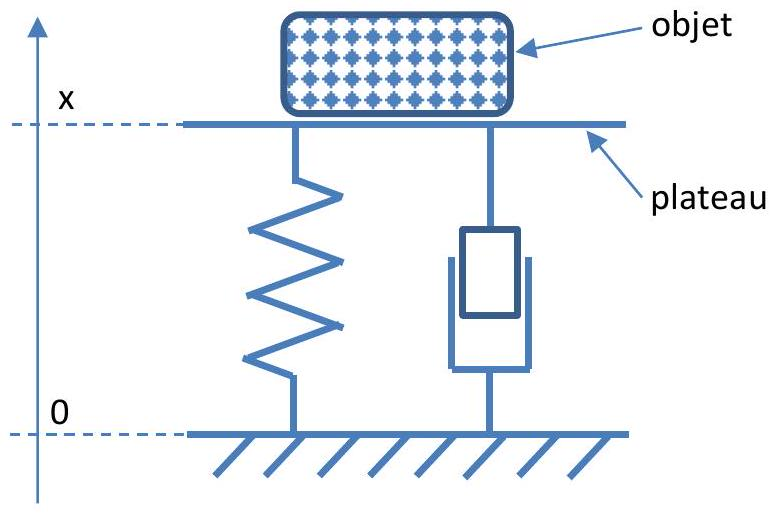
\includegraphics[max width=\textwidth, alt={}]{d2ec2b26-f4f5-41e6-b49c-07a5964b182b-1_531_779_1930_199}
 & \begin{tabular}{l}
L'équation différentielle qui régit la position du plateau en fonction du temps est obtenue en appliquant le PFD : \( \frac{d^{2} x}{d t^{2}}=\frac{k}{m}(l-x)-\frac{\mu}{m} \frac{d x}{d t}-g \) \\
Avec : \\
k : raideur du ressort \\
m : masse de l'objet \\
I : longueur à vide du ressort \\
\(\mu\) : coefficient d'amortissement \\
g : accélération de la pesanteur \\
\end{tabular} \\
\hline
\end{tabular}
\end{center}

A \(\mathrm{t}=0\), on pose l'objet sur le plateau, ce qui donne les conditions initiales suivantes :\\
\(x(t=0)=l \quad ; \quad \frac{d x}{d t}(t=0)=0\)

\begin{enumerate}
  \item En posant \(y(t)=x^{\prime}(t)\), discrétiser le problème en utilisant le schéma d'Euler Explicite :\\
\(X_{n+1}=X_{n}+h f\left(t_{n}, X_{n}\right), \mathrm{h}\) désigne le pas de temps\\
Avec : \(X_{n}=\left[\begin{array}{l}x_{n} \\ y_{n}\end{array}\right]\), et les conditions initiales \(X_{0}=\left[\begin{array}{l}x_{0}=l \\ y_{0}=0\end{array}\right]\)
  \item En utilisant les valeurs numériques suivantes, donner les 2 valeurs de x et de y aux deux premiers instants.\\
\(\mathrm{k}=50 \mathrm{~N} / \mathrm{m} ; \mathrm{m}=0.5 \mathrm{~m} ; \mathrm{I}=0.4 \mathrm{~m} ; \mu=1.5 \mathrm{Ns} / \mathrm{m} ; \mathrm{g}=9.81 \mathrm{~m} / \mathrm{s}^{2}\)\\
Le pas de temps constant sera de \(h=0.01 s\).
  \item Discrétiser le problème en utilisant le schéma de Runge-Kutta d'ordre 2 :\\
\(X_{n+1}=X_{n}+\frac{h}{2}\left(K_{1}+K_{2}\right) \quad\) avec \(\left\{\begin{array}{c}K_{1}=f\left(t_{n}, X_{n}\right) \\ K_{2}=f\left(t_{n}+h, X_{n}+h K 1\right)\end{array}\right.\)
\end{enumerate}

\section*{Exercice 3:}
On exerce sur une poutre un chargement uniforme d'intensité \(q\) et une force axiale \(T\). Le déplacement \(y\) est régit par I'EDP stationnaire suivante :

\[
\left.\left(\frac{d^{2} y}{d x^{2}}\right)-\frac{T y}{E I_{z}}=\frac{q x(L-x)}{2 E I_{z}} \quad \text { pour } x \in\right] 0, L[
\]

avec :\\
\(x=\) Emplacement le long de la poutre (m)\\
\(T=\) Tension appliquée (N)\\
\(E=\) Module de Young (Pa)\\
\(I_{z}=\) Moment quadratique de la poutre \(\left(\mathrm{m}^{4}\right)\)\\
\(q=\) Intensité de la charge uniforme ( \(\mathrm{N} / \mathrm{m}\) )\\
\(L=\) Longueur de la poutre (m)\\
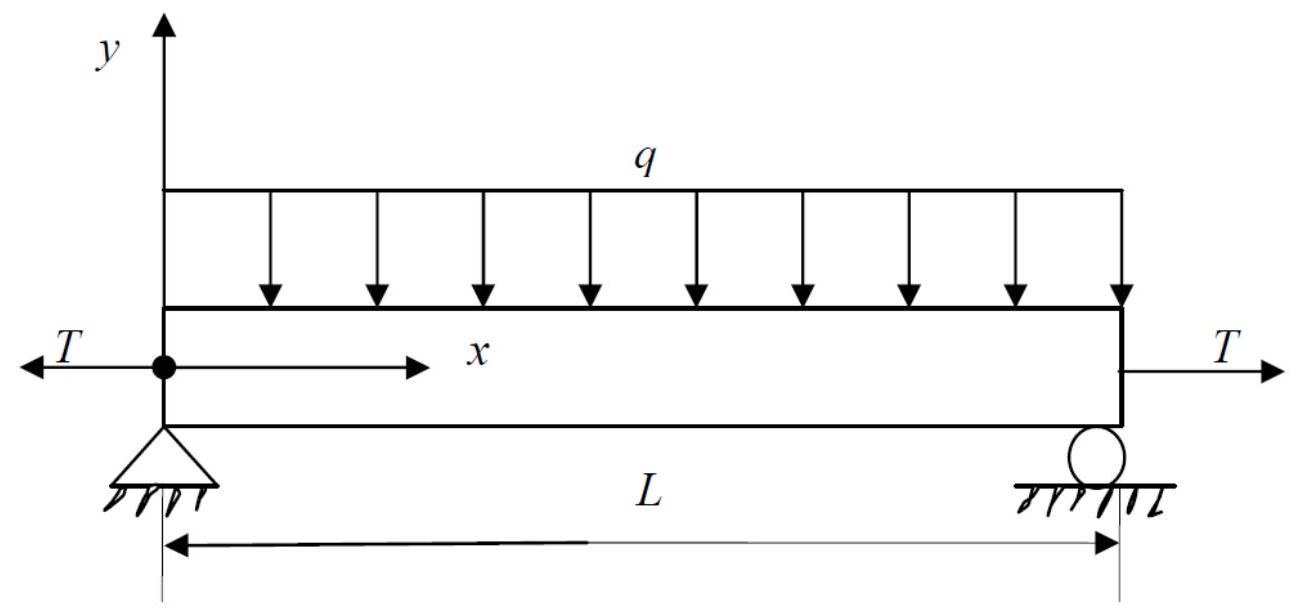
\includegraphics[max width=\textwidth, alt={}, center]{d2ec2b26-f4f5-41e6-b49c-07a5964b182b-2_615_1301_1592_223}

On suppose négligeable (donc nulle) la déformation de la poutre dans l'axe x .\\
On a \(T=2100 \mathrm{~N}, q=12600 \mathrm{~N} / \mathrm{m}, L=12 \mathrm{~m}, \mathrm{E}=210 \mathrm{e} 9 \mathrm{~Pa}\) et \(I_{z}=0.0001 \mathrm{~m}^{4}\).

\begin{enumerate}
  \item Etablir le schéma aux différences finies centré d'ordre 2 pour la dérivée seconde à l'aide de 3 points, puis de 5 points.
  \item Mettre l'équation différentielle sous forme indicielle (discrétisée) à partir d'un schéma numérique centré aux différences finies. Expliquez la démarche.
  \item Donner les conditions aux limites.
  \item Donner l'équation matricielle sur 7 points répartis uniformément sur la poutre \([0, L]\).
  \item Trouver le déplacement de la poutre à 8 m .
  \item La solution exacte de l'EDP précédente est donnée par la fonction suivante :\\
\(y(x)=C_{1} \exp (x / 100)+C_{2} \exp (-x / 100)+3 x^{2}-36 x+60000\)\\
Avec \(C_{1}\) et \(C_{2}\) des constantes à calculer en fonction des conditions aux limites présentes sur le schéma. exp est la fonction exponentielle. Trouver l'erreur relative de calcul de \(y(8)\)
\end{enumerate}

L'erreur relative est donnée par la relation suivante : \(\quad E(\%)=\frac{\left|y_{\text {exacte }}-y\right|}{\left|y_{\text {exacte }}\right|} \times 100\)


\end{document}